\documentclass[onecolumn,10pt]{article}
\usepackage[english]{babel}
\usepackage{times}
\usepackage{graphicx}
\usepackage{amssymb,amsmath}
\usepackage{dsfont}
\usepackage{hyperref}
\usepackage {graphicx}
\usepackage {xspace}
\usepackage{mathtools}
\usepackage[dvipsnames]{xcolor}
\usepackage{enumitem}

%\input ../../lectures/notation.tex

\usepackage[margin=0.6in,foot=0.25in,nohead]{geometry}
\newcommand{\Rx}[1]{\mathds{R}^{#1}}
\newcommand{\ie}{\emph{i.e.} \xspace}
\newcommand{\eg}{\emph{e.g.} \xspace}
\newcommand{\etc}{\emph{etc.} \xspace}

\def\captionfonts{{\em}}
\makeatletter  % Allow the use of @ in command names
\setlength{\abovecaptionskip}{0.3ex plus 0.3ex minus 0.3ex}
\setlength{\belowcaptionskip}{0.3ex plus 0.3ex minus 0.3ex}
\long\def\@makecaption#1#2{%
  \vskip\abovecaptionskip
  \sbox\@tempboxa{{\captionfonts #1: #2}}%
  \ifdim \wd\@tempboxa >\hsize
    {\captionfonts #1: #2\par}
  \else
    \hbox to\hsize{\hfil\box\@tempboxa\hfil}%
  \fi
  \vskip\belowcaptionskip}

\renewcommand\section{\@startsection{section}{1}{\z@}%
                       {-1.8ex \@plus -0.8ex \@minus -0.8ex}%
                       {1ex \@plus 0.4ex \@minus 0.4ex}%
                       {\normalfont\large\bfseries\boldmath
                        \rightskip=\z@ \@plus 8em\pretolerance=10000 }}
\renewcommand\subsection{\@startsection{subsection}{2}{\z@}%
                       {-1.0ex \@plus -0.6ex \@minus -0.6ex}%
                       {1.0ex \@plus 0.3ex \@minus 0.3ex}%
                       {\normalfont\normalsize\bfseries\boldmath
                        \rightskip=\z@ \@plus 8em\pretolerance=10000 }}

\makeatother   % Cancel the effect of \makeatletter


\setlength{\parindent}{0in}
\setlength{\parskip}{1.5ex}

%\long\def\solution#1{\textit{Solution:}\\
%\begin{tabular}{@{\hspace{1ex}}|@{\hspace{1ex}}p{6in}}
%{\begin{minipage}{\linewidth}#1\end{minipage}} \end{tabular}}

%\long\def\solution#1{#1}
\long\def\solution#1{}


%%% for tracking points per question
\usepackage{pgfkeys}
\pgfkeys{
 /points array/.is family, /points array,
 .unknown/.style = {\pgfkeyscurrentname/.initial = #1},
}

\newcommand\questionhaspoints[1]{\pgfkeys{/points array, #1}}
\newcommand\getquestionpoints[1]{\pgfkeysvalueof{/points array/#1}}

% for code formatting
\usepackage{listings,color}
\definecolor{verbgray}{gray}{0.9}
\lstnewenvironment{code}{%
  \lstset{backgroundcolor=\color{verbgray},
  frame=single,
  framerule=0pt,
  language=bash,
  basicstyle=\ttfamily,
  columns=fullflexible}}{}

\begin{document}

%Title here
\vspace{0mm}
\textbf{\large ROB 498/599 3D Robot Perception: HW1 Writeup Template}\\
\textbf{Name:} Your Name Here\\
\textbf{Uniqid:} Your Uniqid Here \\
\textbf{Email:} Your Email here \\

\vspace*{1mm}
\hrule
\vspace*{1mm}

\noindent
\vspace{1mm}

\noindent
%\textbf{Data:} You need to download the supplemental data to complete this assignment.  All paths in the assignment assume the data is off the local directory.  The download has data and code; it is named \texttt{hw1.zip}.  \vspace{1mm}


\newcounter{problemnumber}
\setcounter{problemnumber}{0}

\questionhaspoints{0=0,1=20,2=20,3=20,4=10,5=20,6=10}


\noindent\textbf{Instructions: }
Each bullet point in this template contains the prompt for what information should be included in the write up. Replace the bullet point with your own answer to the question/prompt described in the bullet point. Finally, submit a \texttt{.zip} file containing this write-up and a folder \texttt{scripts} with all the python scripts on Canvas.

\addtocounter{problemnumber}{1}
\noindent\textbf{Problem \arabic{problemnumber}}: Camera Calibration

 i. In this paragraph, briefly describe the camera calibration process as implemented in your code. How did you obtain your projection matrix? How did you verify it was correct? If you were provided with a different pair of images, how would you obtain projection matrices for the new cameras? In equation \ref{eq:projection_matrix}, report the projection matrix you obtained from your code to 4 significant figures.


\begin{align}
M=\begin{bmatrix}
0.0011 & 0.0012 & 0.0013 & 0.0014 \\
0.0021 & 0.0022 & 0.0023 & 0.0024 \\
0.0031 & 0.0032 & 0.0033 & 0.0034 \\
\end{bmatrix}
\label{eq:projection_matrix}
\end{align}


ii. In this paragraph, describe your reprojection error results. What does this error represent? What units is it in? If you were provided with a different pair of images and had to recreate this process, how would you validate that your re-projection error was okay? Report the reprojection error of your obtained projection matrix in equation \eqref{eq:reprojection_error} to 6 significant figures.


\begin{equation}
errror_{reprojection}=1.23456 \label{eq:reprojection_error}
\end{equation}

\noindent\textbf{Sparse 3D Reconstruction}


\addtocounter{problemnumber}{1}
\noindent\textbf{Problem \arabic{problemnumber}}:  Estimation of Fundamental Matrix

i. Briefly discuss the fundamental matrix - what does it actually represent, and how did you obtain it? Report your obtained fundamental matrix to 4 significant figures below in equation \ref{eq:fundamental_matrix}.

\begin{align}
F=\begin{bmatrix}
0.0011 & 0.0012 & 0.0013 \\
0.0021 & 0.0022 & 0.0023 \\
0.0031 & 0.0032 & 0.0033 \\
\end{bmatrix}
\label{eq:fundamental_matrix}
\end{align}

\begin{figure}[h]
  \centering
  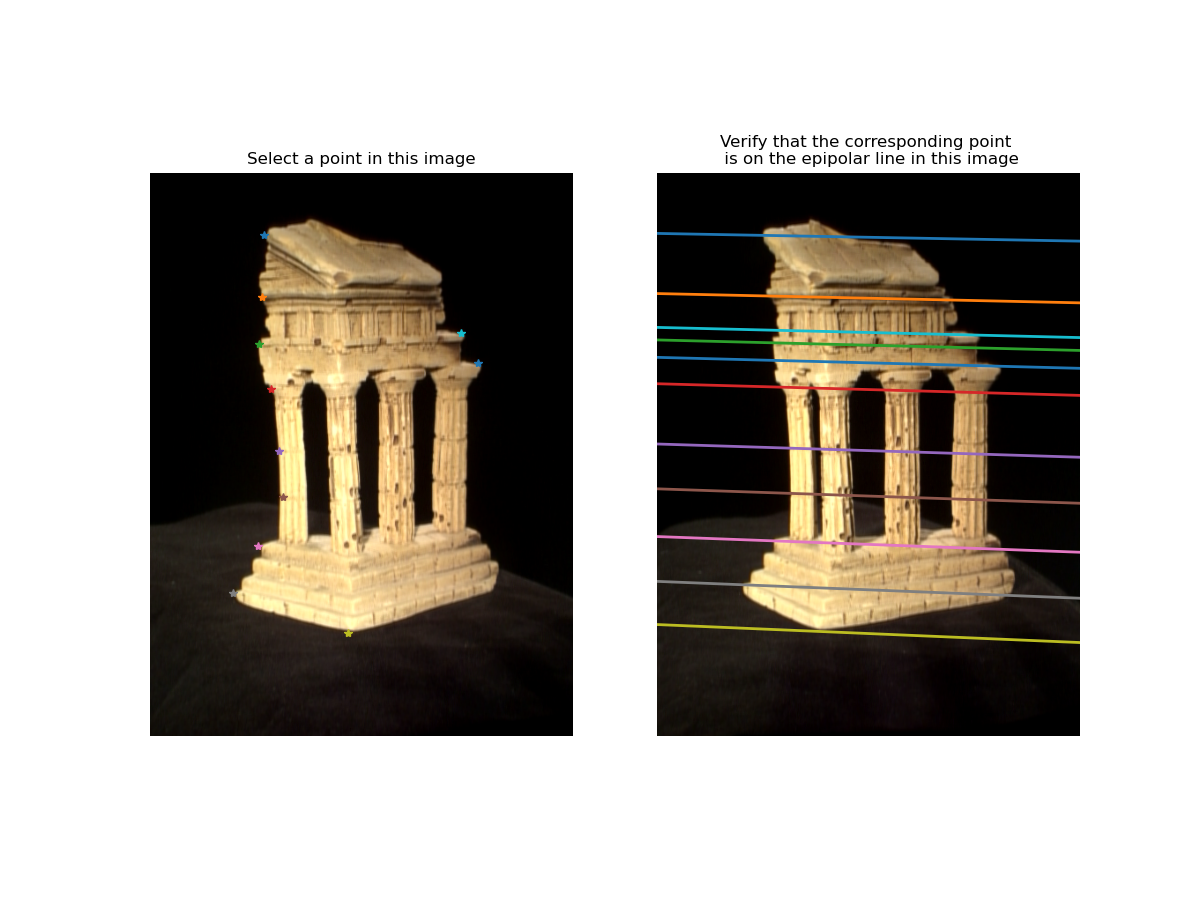
\includegraphics[width=0.66\textwidth]{media/Epipolar line.png}
  \caption{Sample image for GUI output for epipolar lines \textit{(Students: update this caption with a better description prior to submission)}}
  \label{fig:epipolar lines}
\end{figure}

ii. Discuss how you validated your fundamental matrix. Replace the image in figure \ref{fig:epipolar lines} with a screenshot of your{\tt  epipolar\_lines\_GUI\_tool} results containing at least 6 selected points and reference it here. Were all of the points equally accurate? How did you verify that the drawn epipolar lines were correct? What sources of error exist that may cause these epipolar lines to not be correct?



\addtocounter{problemnumber}{1}
\noindent\textbf{Problem \arabic{problemnumber}}:  Find Epipolar Correspondences

i. Discuss the process for finding correspondances between the two images. What function did you use for your similarity? How did it work? Did you experiment with any other similarity functions, or experiment with any of the parameters (patch size, etc.) of your final function? If so, report on what you tried, and what made you choose your final submitted function.

ii. Replace the image in figure \ref{fig:epipolar_corresp} with a screenshot of your {\tt epipolar\_correspondences\_GUI\_tool} results containing at least 6 selected points and reference here. Which correspondences in your image had the best and worst results? What sources of error exist for your correspondance determination process, and how might they be address going forward?

\begin{figure}
  \centering
  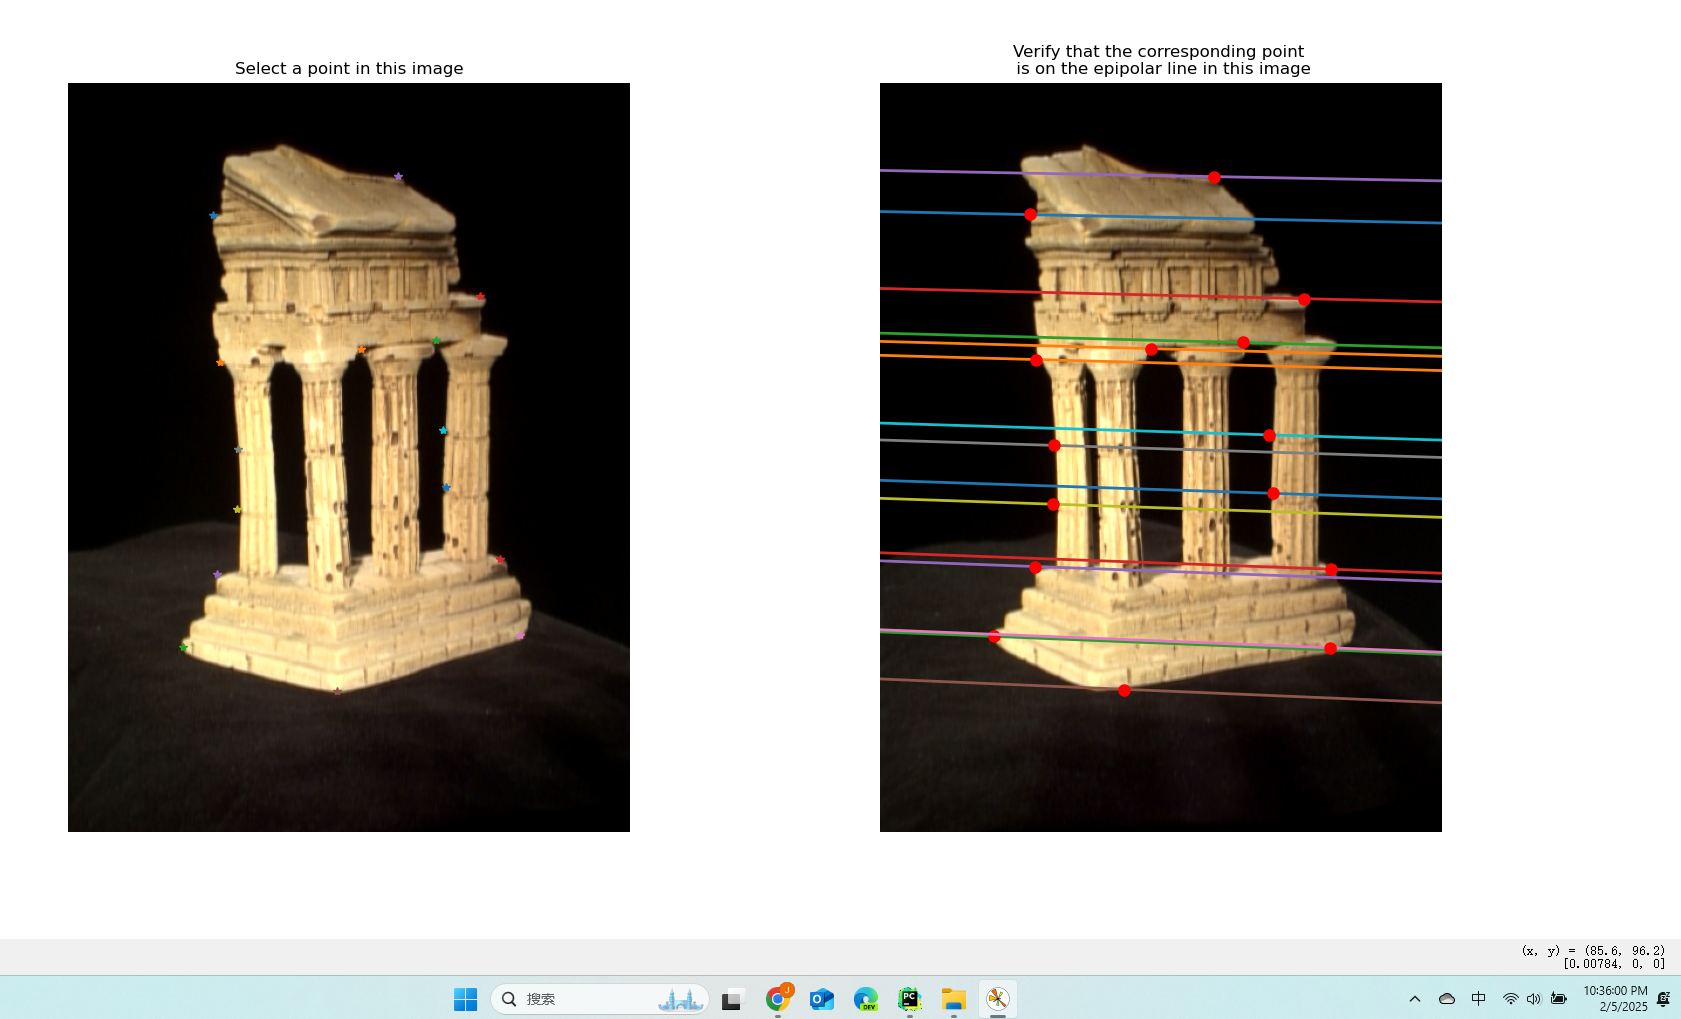
\includegraphics[width=0.66\textwidth]{media/Epiploar correspondence.png} % Replace with your image file name and extension
  \caption{Sample image for GUI output for epipolar correspondences \textit{(Students: update this caption with a better description prior to submission)}}
  \label{fig:epipolar_corresp}
\end{figure}

\addtocounter{problemnumber}{1}
\noindent\textbf{Problem \arabic{problemnumber}}:  Compute the Essential Matrix

i. Discuss the essential matrix calculation. Briefly discuss the equation/derivation for obtaining the essential matrix from the fundamentals and the intrinsics. What does the essential matrix represent? Report your obtained essential matrix to 4 significant figures below in equation \ref{eq:essential_matrix}.

\begin{align}
E=\begin{bmatrix}
0.0011 & 0.0012 & 0.0013 \\
0.0021 & 0.0022 & 0.0023 \\
0.0031 & 0.0032 & 0.0033 \\
\end{bmatrix}
\label{eq:essential_matrix}
\end{align}

\addtocounter{problemnumber}{1}
\noindent\textbf{Problem \arabic{problemnumber}}:  Triangulation

i. Discuss the process for determining the correct extrinsic matrix. After decomposition, how did you determine which extrinsic matrix was correct - what did you look at? If you automated this process, descibe your algorithm. Report the determined extrinsic matrix below in equation \ref{eq:extrinsic_matrix} to 4 significant figures.

\begin{align}
Ext=\begin{bmatrix}
0.0011 & 0.0012 & 0.0013 \\
0.0021 & 0.0022 & 0.0023 \\
0.0031 & 0.0032 & 0.0033 \\
\end{bmatrix}
\label{eq:extrinsic_matrix}
\end{align}


ii. Discuss the setup of the SVD problem - what did the final equations you used look like to determine the $A$ matrix? Report and discuss your reprojection error to 6 significant figures in equation \ref{eq:reprojection_error_3d}. What does this error represent? What units is it in?

\begin{equation}
errror_{reprojection3d}=1.23456 \label{eq:reprojection_error_3d}
\end{equation}

iii. Discuss any differences between your approach and OpenCV's approach. Are the resulting reprojection errors different? What could be the source of these differences? Report and discuss the OpenCV reprojection error to 6 significant figures in equation \ref{eq:reprojection_error_ocv}. What does this error represent? What units is it in?

\begin{equation}
errror_{reprojectionOCV}=1.23456 \label{eq:reprojection_error_ocv}
\end{equation}


\addtocounter{problemnumber}{1}
\noindent\textbf{Problem \arabic{problemnumber}}:  Connecting the dots and visualizing the point cloud

i. Discuss the program flow you implemented for the main function - what were the steps you took to perform 3d reconstruction in general?

ii. Discuss the \texttt{visualize(point\_cloud)} function you implemented. How does it work, and what steps did you take to verify its output?

iii. Replace the image in figure \ref{fig:reconstruction} with a screenshot of your 3d visualization results. Discuss your output - does it look correct to you? Are all of the points in their correct locations? Discuss the accuracy of the point locations and potential sources of error in this representation.

\begin{figure}
  \centering
  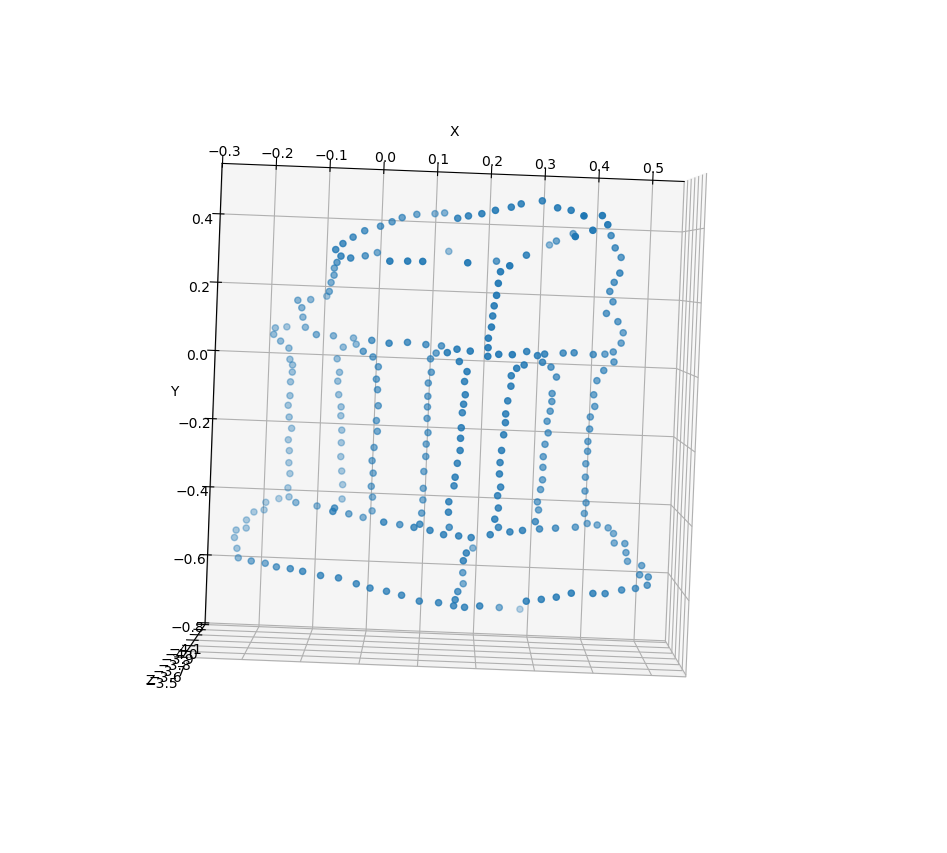
\includegraphics[width=0.4\textwidth]{media/Reconstruction.png} % Replace with your image file name and extension
  \caption{Sparse Reconstruction \textit{(Students: update this caption with a better description prior to submission)}}
  \label{fig:reconstruction}
\end{figure}


\addtocounter{problemnumber}{1}
\noindent\textbf{Optional Problem \arabic{problemnumber}}: Pain points and Flash cards

i. If you had any particular difficulties in the homework, or had any extra figures, experiments, etc. you would like to show off, feel free to discuss them here.



\noindent\textbf{References and Credits:}\\
Parts of this homework are from David Fouhey's EECS 442 and CMU 16-385, and from Jason Corso's ROB 498/599 classes.

\end{document}